\chapter{Deep Net} \label{cap1}
In questo capitolo si mostra come è stato creato il dataset per l'addestramento della Deep Net e la sua struttura.
\section{Training Set}
Nel primo lavoro, Bourdev come campioni di addestramento per ogni tipo di poselet ha utilizzato un dataset chiamato \textit{H3D} presentato nella medesima pubblicazione. In questo dataset vengono etichettate alcune zone particolari del corpo umano (naso, occhio destro/sinistro, orecchie, spalle etc.) come \textit{keypoints}. Una poselet è una regione dell'immagine dove sono presenti keypoints con una specifica configurazione spaziale. Quindi ad esempio possiamo avere una poselet relativa alla faccia vista in posizione frontale, oppure una poselet relativa alla parte superiore del corpo sempre vista in posizione frontale

\begin{figure}[h!b]
 \centering
 \subfloat {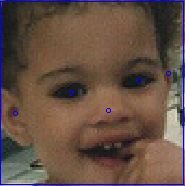
\includegraphics[width=4cm]{cap1/poselet1.jpg}}
 \hspace{5mm}
 \subfloat {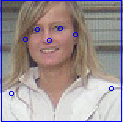
\includegraphics[width=4cm]{cap1/poselet2}}
 \caption{A sinistra poselet con 5 keypoints, a destra 7 keypoints}
 \end{figure}
 
 Nel primo lavoro basato su HOG, per ogni tipo di poselet (sono stati estratti 150 tipi di poselets\cite{poselets-image}) vengono raccolti i campioni utilizzando le immagini presenti nel dataset H3D.\\
 In questo approccio utilizziamo una CNN come estrattore di caratteristiche.
 
 \begin{figure}[h!b]
 \centering
 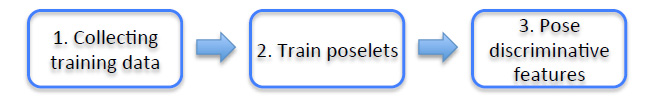
\includegraphics[scale=0.5]{cap1/train}
 \caption{Fasi di addestramento della Deep Net}
 \label{}
 \end{figure}
 
 
 
 Uno dei problemi maggiori che affligge l'utilizzo delle CNN è che necessitano di un numero enorme di campioni di addestramento per evitare il fenomeno dell'overfitting. Le immagini presenti nel dataset H3D non bastano e quindi viene presentato un approccio per ottenere il numero necessario di campioni.\\
 E' stato utilizzato il software pubblicamente disponibile\cite{poselet-code} relativo al primo lavoro di Bourdev sulle poselets utilzzando HOG come estrattore di caratteristiche. Come dataset è stato utilizzato COCO\cite{coco} il quale contiene circa 50000 immagini di persone con relative ground truth. Sono stati estratti i bounding boxes individuati dal software: ciascun bounding box è supportato da un insieme di attivazioni-poselet le quali sono etichettate positive se il bounding box relativo e la ground truth danno un intersection-over-union di almeno 0.5, altrimenti negative.
 
\begin{figure}[h!b]
\centering
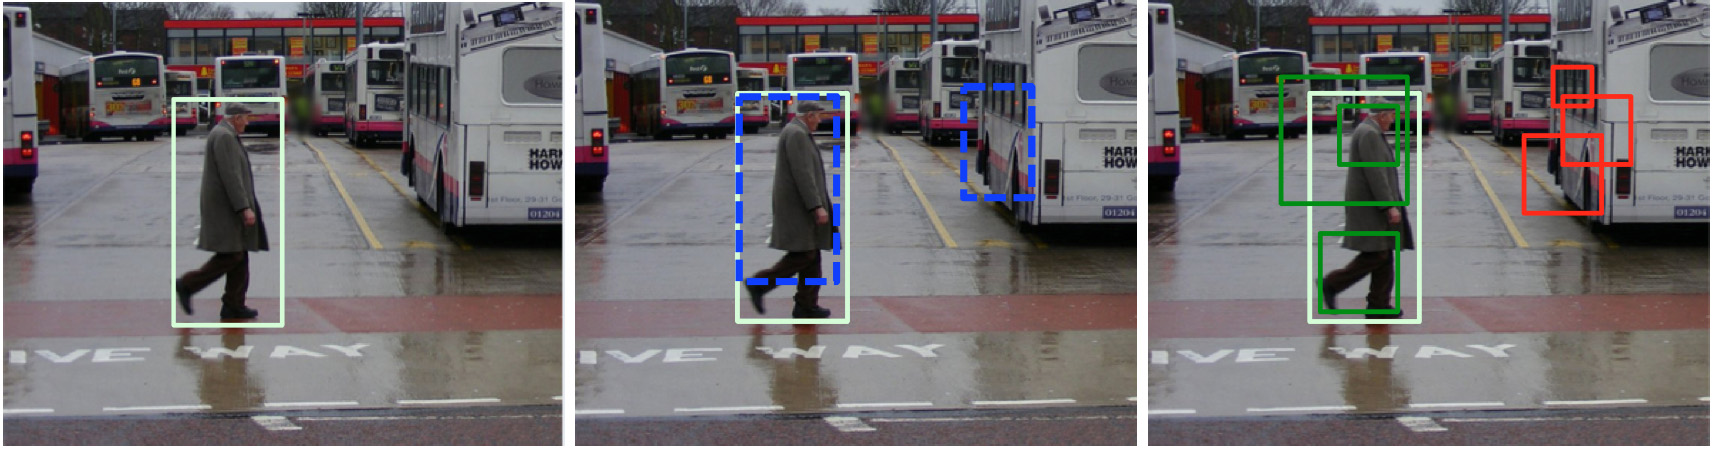
\includegraphics[scale=0.25]{cap1/act_label}
\caption{\textbf{Sinistra:} persona con relativa ground truth \textbf{Centro:} in blu bounding boxes rilevati \textbf{Destra:} in verde attivazioni positive, in rosso negative }
\label{}
\end{figure}

Il metodo illustrato permette di ottenere circa 20000 immagini per ciascun tipo di poselet, per un totale di 3 milioni di campioni positivi. Si ottengono inoltre circa 2 milioni di immagini di background.

\section{Deep Net}
Nella tabella \ref{table-deepnet} viene mostrata la struttura della Deep Net. L'input è una patch RGB di dimensioni 61x61x3 estratta tramite ridimensionamento dalle attivazioni-poselet: ad esse è stata sottratta la media. 

\begin{table}[h!b]
\centering
\begin{tabular}{|l | c | c | c | c | c | c|}
 \hline
 Layer & 1 & 2 & 3 & 4 & 5 & 6 \\ \hline
 Stage & conv+max & conv & conv & conv & full & full \\ \hline
 \#channels & 64 & 256 & 128 & 128 & 256 & 5 \\ \hline
 Filter Size & 5x5 & 5x5 & 3x3 & 3x3 & - & - \\ \hline
 Conv Stride & 2x2 & 1x1 & 1x1 & 1x1 & - & - \\ \hline
 Pooling Size 3x3 & - & -& -& -& - & -\\ \hline
 Pooling Stride 2x2 & - & -& -& -& - & - \\ \hline
 Zero Padding Size - & - & -& -& -& - & - \\ \hline 
 Spacial input size & 61x61x3 & 14x14 & 10x10 & 8x8 & 6x6 & 1x1 \\
 \hline
\end{tabular}
\caption{Struttura Deep Net}
\label{table-deepnet}
\end{table}

Visto l'enorme onere computazionale, in questa implementazione al posto di classificare una patch tra 151 classi (150 tipi di poselet più background) si è scelto di utilizzare un numero di classi pari a 5 (4 tipi di poselets e background). Quindi la prima classe corrisponde al tipo poselet 16, la seconda classe il tipo 144, la terza il tipo 97 e la quarta il tipo 86. Ricordiamo che è possibile vedere i vari tipi di poselets al seguente link\cite{poselets-image}.

\begin{figure}[h!b]
 \centering
 \subfloat {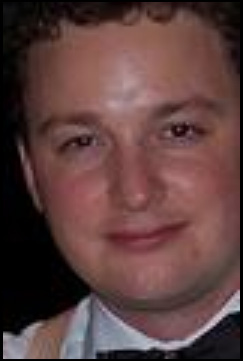
\includegraphics[width=3cm]{cap1/pos11}}
 \hspace{3mm}
 \subfloat {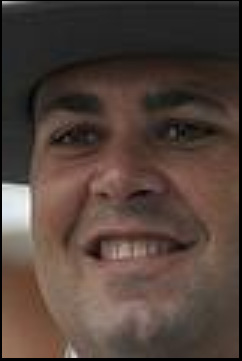
\includegraphics[width=3cm]{cap1/pos12}}
 \hspace{3mm}
 \subfloat {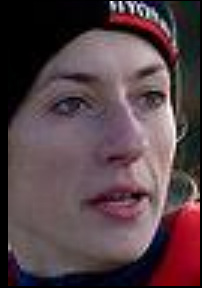
\includegraphics[width=3cm]{cap1/pos13}}
 \hspace{3mm}
 \subfloat {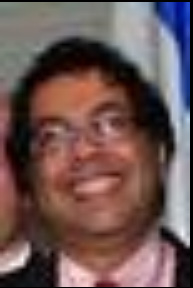
\includegraphics[width=3cm]{cap1/pos14}}
 \caption{Esempi di immagini della prima classe (\#poselet 16)}
 \end{figure}
 
 \begin{figure}[h!b]
 \centering
 \subfloat {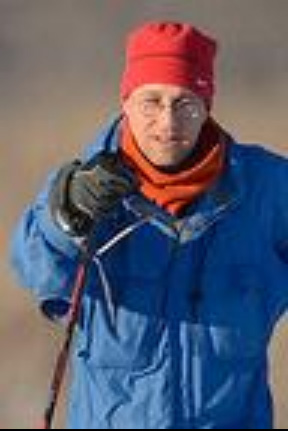
\includegraphics[width=3cm]{cap1/pos21}}
 \hspace{3mm}
 \subfloat {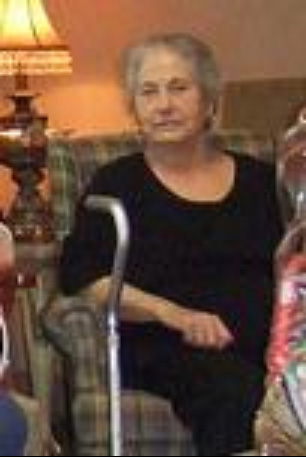
\includegraphics[width=3cm]{cap1/pos22}}
 \hspace{3mm}
 \subfloat {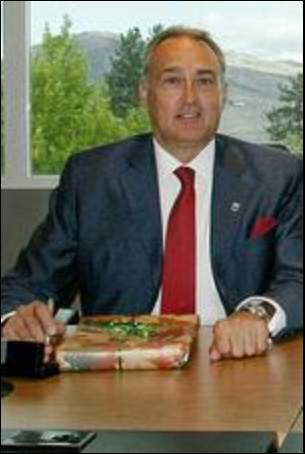
\includegraphics[width=3cm]{cap1/pos23}}
 \hspace{3mm}
 \subfloat {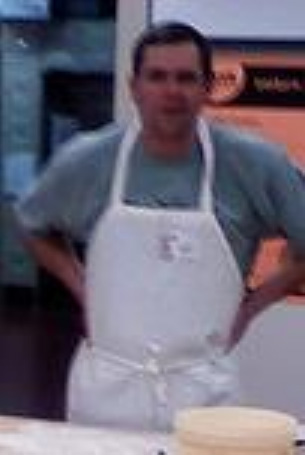
\includegraphics[width=3cm]{cap1/pos24}}
 \caption{Esempi di immagini della seconda classe (\#poselet 144)}
 \end{figure}
 
  \begin{figure}[h!b]
 \centering
 \subfloat {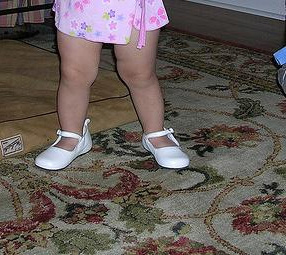
\includegraphics[width=3cm]{cap1/pos31}}
 \hspace{3mm}
 \subfloat {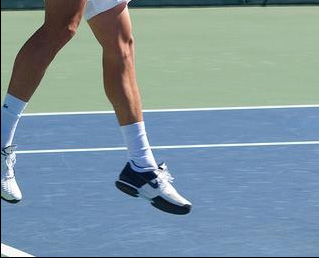
\includegraphics[width=3cm]{cap1/pos32}}
 \hspace{3mm}
 \subfloat {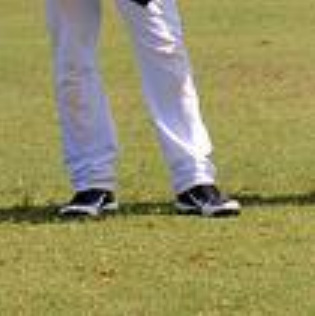
\includegraphics[width=3cm]{cap1/pos33}}
 \hspace{3mm}
 \subfloat {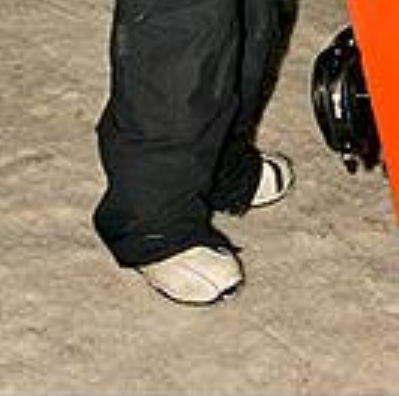
\includegraphics[width=3cm]{cap1/pos34}}
 \caption{Esempi di immagini della terza classe (\#poselet 97)}
 \end{figure}
 
 \begin{figure}[h!b]
 \centering
 \subfloat {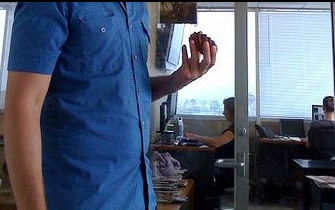
\includegraphics[width=3cm]{cap1/pos41}}
 \hspace{3mm}
 \subfloat {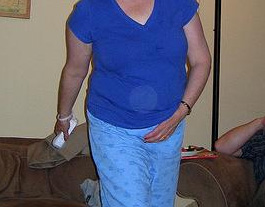
\includegraphics[width=3cm]{cap1/pos42}}
 \hspace{3mm}
 \subfloat {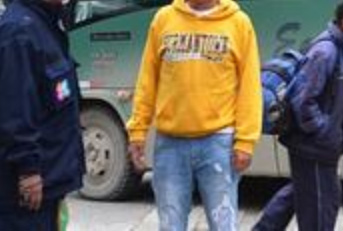
\includegraphics[width=3cm]{cap1/pos43}}
 \hspace{3mm}
 \subfloat {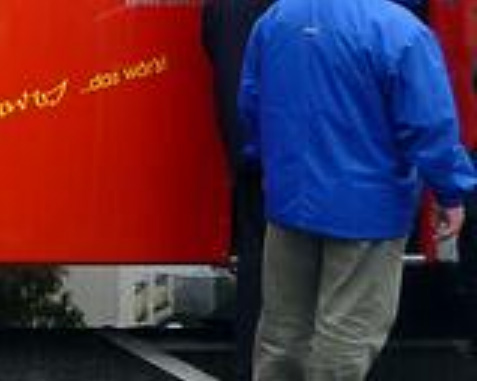
\includegraphics[width=3cm]{cap1/pos44}}
 \caption{Esempi di immagini della quarta classe (\#poselet 86)}
 \end{figure}
 
 Le immagini sono state divise in 72 batch, ognuno contenente 250 campioni positivi per ogni classe e 700 negativi: in totale sono state processate 122400 immagini campione. Il learning rate iniziale è stato impostato a 0.15, utilizzando il valore 1e-5 per il weigth-decay e 0.9 per il momentum.


\begin{figure}[h!b]
\centering
  
  \[\Delta w_i(t+1)=w_i-n\frac{\delta E}{\delta w_i}+\alpha \Delta w_i(t) -\lambda \eta w_i \]
  \caption{Aggiornamento Parametri. ${\alpha}$  momentum. ${\lambda}$ weight-decay. ${\eta}$ learning-rate}
\end{figure}
 
L'utilizzo del weight-decay penalizza i grossi cambiamenti di parametri tra un passo e l'altro, mentre il momentum permette di diminuire le fluttuazioni dei cambiamenti di parametri tra un iterazione e l'altra. Si è riusciti ad ottenere un errore di classificazione di circa il 9\% su un validation-set composto da 600 campioni: 150 campioni positivi per ogni classe e 150 campioni negativi.
 
 
 
 